\documentclass[11pt,a4paper]{article}
\usepackage[T1]{fontenc}
\usepackage[utf8]{inputenc}
\usepackage{times}
\usepackage[margin=2.4cm]{geometry}
\usepackage{graphicx}
\usepackage{booktabs}
\usepackage{amsmath}
\usepackage{url}
\usepackage[colorlinks=true,linkcolor=black,citecolor=black,urlcolor=blue]{hyperref}
\usepackage{microtype}
\usepackage{caption}
\captionsetup{font=small,labelfont=bf}
\urlstyle{same}
\setlength{\parskip}{4pt}

\title{\LARGE Self Supervised Learning for Forest Clear Cut Detection: Training Budgets, Label Budgets and Spatial Validation on Sentinel 2 Time Series}
\author{Nida Kumbasar$^{1}$ \and Mehmet Oğuz Güneren$^{2}$\\[6pt]
\small $^{1}$TÜBİTAK BİLGEM, Information Technologies Institute (BTE), Data Valorization Department, Gebze, Kocaeli, Türkiye \\
\small \texttt{nida.kumbasar@tubitak.gov.tr}\\[3pt]
\small $^{2}$Department of Artificial Intelligence and Data Engineering, Istanbul Technical University, Istanbul, Türkiye \\
\small \texttt{gnrnoguz@gmail.com}}
\date{\small Draft for coauthor review \textbullet{} 18 October 2026 \textbullet{} Version paper\_v4 with declared extensions paper\_v5 and paper\_v6}

\begin{document}
\maketitle

\begin{abstract}
Self supervised pretraining may improve satellite time series classification when labels are scarce, but comparisons can confound its objective with additional optimization. This issue is examined using 2,213 high confidence DISFOR Sentinel 2 series, comprising 1,937 stable forest and 276 clear cut locations. A fixed protocol evaluates random forests, temporal convolutional networks, supervised Transformers and masked reconstruction Transformers with five spatially grouped folds, three training seeds and two label budgets. Spatial components connect locations within 5 km and shared source disturbance events. All 180 fits are retained. At 20\% labels, block and band pretraining achieves pooled out of fold macro F1 0.8690, compared with 0.8322 for a 40 epoch supervised Transformer; the paired difference is 0.0368 (conditional spatial component bootstrap 95\% interval [0.0245, 0.0506]). However, a supervised control approximately matching the total optimizer step budget reaches 0.8987. Independent cell masking reaches 0.8609, and the corresponding masking comparison does not clearly separate the methods. With all labels, the CNN reaches 0.9299 and the pretrained Transformer 0.9287. Two declared extensions qualify this picture. A label budget curve at 5\%, 10\% and 50\% labels on the identical folds and seeds shows that below 20\% labels the pretrained Transformer trails the step matched Transformer, the CNN and even the random forest, so its benefit is confined to the short training comparison; at 50\% labels the neural recipes converge. A single seed grouping radius analysis at 5, 10 and 20 km shows that the step matched advantage does not persist under coarser spatial separation, where the pretrained model degrades least. Metadata and missingness controls expose residual sampling information. Because the recipes were developed on the same dataset, the study is a retrospective audit and does not constitute external validation. An unused location support audit yields only one positive among 111 eligible windows and is therefore not scored. These results support optimization aware, spatially structured evaluation and do not support a general claim of self supervised superiority.

\end{abstract}
\noindent\textbf{Keywords:} Earth observation; Sentinel 2; forest disturbance; self supervised learning; spatial validation; optimization controls

Draft for co author review \textbullet{} 18 October 2026 \textbullet{} Version paper\_v4 with declared extensions paper\_v5 (grouping radius) and paper\_v6 (label budget curve)

\section{Introduction}
Dense satellite time series offer observations of vegetation before and after disturbance, whereas reliable event labels remain costly to obtain. Self supervised learning can use observations without their class labels before supervised adaptation. This motivates a practical question: when a pretrained classifier improves under a limited label budget, how much of that improvement survives a stronger supervised comparator? A useful answer requires both geographically separated evaluation and explicit control of additional training.

Masked representation learning for multivariate time series is established prior work \cite{ref3}. In Earth observation, lightweight pretrained temporal models such as Presto already demonstrate the broader relevance of time series pretraining \cite{ref7}. Zhang et al. apply a self supervised Transformer to Sentinel 1 and Sentinel 2 time series for forest disturbance type detection in a subtropical ecosystem \cite{ref2}. Resampling based contrastive augmentation has also been examined for remote sensing sequences \cite{ref8}. These studies motivate the present questions; their datasets, objectives and metrics are not directly comparable to this experiment. None of those systems is reproduced here, and no new Transformer architecture or state of the art result is claimed.

Forest disturbance mapping from optical time series has a long record, from global Landsat based cover change products \cite{ref17} and continuous change detection \cite{ref20} to European disturbance regime maps \cite{ref18} and reviews of optical disturbance and degradation methods \cite{ref19}; a recent global disturbance type dataset extends this line \cite{ref24}. Deep sequence models for satellite image time series include temporal convolutions \cite{ref11}, self attention over raw optical sequences \cite{ref12} and pixel set temporal attention encoders \cite{ref13}. Self supervised pretraining for such sequences has followed the masked token recipe of language and vision models \cite{ref14}, with SITS BERT \cite{ref9}, SITS Former \cite{ref10}, SatMAE \cite{ref15}, Presto \cite{ref7} and generalist geospatial foundation models \cite{ref16} as representative examples; multimodal Sentinel 1/2 fusion is also common in the applied literature \cite{ref25,ref26}. The methodological concern that motivates the present design is that random cross validation can overstate map accuracy under spatial dependence \cite{ref4,ref21,ref22}, although the appropriate design depends on the intended inference target \cite{ref23}.

A restricted binary subset of DISFOR, a public European disturbance time series resource \cite{ref1}, is used. Structured dependence can compromise ordinary cross validation, making spatial and event grouping relevant \cite{ref4}. Yet spatial separation alone does not resolve training budget imbalance, missingness cues or dataset specific model development. The contribution is a reproducible empirical audit that reports these issues together: paired label subsets, fixed training recipes, an optimization step control, a masking control, covariate only diagnostics and an explicit audit of unused evaluation support. The central comparison was fixed before the new cross fit scores were computed; the architecture choices had already been explored on this dataset.

\section{Data and study design}
JR DIGITAL/DISFOR is pinned to revision 2562332e35c94c2339aeb341ffaed2a99faae7d6. The downloaded sample table contains 3,822 locations; an upstream dataset card count of 3,823 is not used. DISFOR provides interpreted labels and Sentinel 2 observations, with source campaigns involving disturbance polygons, sampling strata and storm event information. The dataset article is an ESSD Discussions preprint under review at the time of this draft \cite{ref1}. The labels are existing human interpretations supported by ancillary source information; no new field measurements were collected.

High confidence locations are retained and one 24 month calendar window is constructed per location. The first year must be labeled stable forest. A positive window has an eligible clear cut event in its second year; a negative remains stable through both years. Target years range from 2018 to 2023. Candidate event windows are prioritized deterministically, and stable window selection follows the fixed sample identifier rule in the preprocessing code. The task is retrospective classification of curated windows; event onset forecasting and complete landscape mapping are outside its scope. Event dates guide dataset construction but are not input features.

The ten channels are B02, B03, B04, B05, B06, B07, B08, B8A, B11 and B12. Within each month, the median of source clear observations whose scene classification values are 4 or 5 is taken. Each retained window has at least six observed months in each year. Missing values retain a Boolean mask; no temporal interpolation is applied. Values use the source provided digital number scale without an added radiometric offset. Per channel means and standard deviations use observed values from the outer training partition only. Time features encode elapsed days and an annual sine/cosine cycle on monthly calendar slots. Figure 1 shows retained locations and observed month support.

\begin{table}[htbp]
\centering

\caption{Table 1. Sequential selection of the fixed primary cohort.}
\begin{tabular}{lr}
\toprule
Stage & Locations \\ \midrule
Downloaded sample table & 3,822 \\
Exclude non high confidence interpretations & $-$598 \\
Exclude ambiguous or unavailable two year windows & $-$606 \\
Exclude inadequate clear month support & $-$116 \\
Exclude wildfire from the binary primary task & $-$289 \\
Retained stable forest / clear cut & 1,937 / 276 \\
Total retained locations / spatial components & 2,213 / 874 \\
\bottomrule
\end{tabular}
\end{table}

The binary scope was chosen during earlier development after the original held out wildfire class had inadequate support. This prior decision is part of the adaptive development history. The present study does not evaluate fire, disease, mixed disturbance or national transfer. Class prevalence in the retained cohort is 12.47\% clear cut and is not an estimate of landscape prevalence.

An undirected grouping graph joins locations within 5 km and locations sharing a source disturbance event identifier in campaigns 1 or 3. Its connected components are indivisible. Campaign 2 sampling strata are not treated as disturbance event identifiers. Five fold StratifiedGroupKFold uses shuffle=True and random\_state=4192026 over the complete retained cohort. All locations contribute one held out prediction per method and seed. Direct outer training versus outer test proximity was checked after splitting; the smallest distance is 5.0011 km. This threshold prevents nearby cross fold pairs under the specified rule, but it does not establish that all spatial autocorrelation has disappeared.

\begin{table}[htbp]
\centering

\caption{Table 2. Held out support in each fixed fold.}
\begin{tabular}{lrrr}
\toprule
Fold & Stable & Clear cut & Nearest train point (km) \\ \midrule
1 & 385 & 54 & 5.0021 \\
2 & 386 & 54 & 5.0110 \\
3 & 391 & 58 & 5.0011 \\
4 & 386 & 53 & 5.0011 \\
5 & 389 & 57 & 5.0021 \\
\bottomrule
\end{tabular}
\end{table}

\section{Models and experimental controls}
The primary methods are a random forest, a temporal CNN, a supervised Transformer and the same Transformer with masked reconstruction pretraining. The random forest \cite{ref5} has 500 trees, minimum leaf size 4, max\_features=0.7 and balanced\_subsample class weights. Its 60 features comprise per channel observed mean, standard deviation, minimum, maximum, second year minus first year mean and observed fraction. It therefore serves as a temporal summary baseline and uses no spatial context.

Neural inputs concatenate ten normalized values, ten observation indicators and three time features. A linear projection precedes the encoder. The CNN has width 64 and three residual blocks with dilations 1, 2 and 4, each containing two width three convolutions and group normalization. The Transformer has width 48, two encoder layers, four attention heads and feed forward width 144. Both use GELU activations and an observed time mean pooling classifier. Entirely unobserved Transformer keys are masked. CNN dropout is 0.20; Transformer dropout is 0.15. The reconstruction head maps encoded slots to ten channel values.

Primary neural fits use 40 supervised epochs, batch size 64 and AdamW with weight decay 0.01. Learning rates are 0.001 for the CNN and 0.0005 for the Transformer. Cross entropy uses inverse frequency weights calculated from the labeled training subset, label smoothing 0.02 and gradient clipping at norm 1. Training randomly removes months with probability 0.10, restoring the original mask if removal would hide every observation. No early stopping, validation based calibration, model selection or threshold fitting occurs within the new audit. All class decisions use probability 0.5. Reporting a Brier score does not imply a calibrated deployment model \cite{ref6}.

Masked pretraining uses all outer training sequences, without using their class labels in the reconstruction loss, for 60 epochs at learning rate 0.001. Each series hides a contiguous block of two to six months plus two randomly selected complete bands. The loss is Smooth L1 over artificially hidden, originally observed cells. Naturally missing cells are not reconstruction targets. A safeguard retains visible and hidden support. On a fully observed 24 by 10 grid, nominal expected coverage is one third; boundary effects and actual missingness mean that observed cell coverage need not equal one third for every series. After pretraining, the classifier is restored to its paired initial state, and supervised randomization is reset identically across paired methods.

For each seed (7, 17 or 27), labels are sampled in a nested random order separately within each class, using the ceiling of either 20\% or 100\% of the training class count. All methods and controls share these exact point identifiers. Because allocation uses known class membership, the design simulates label scarcity under control and should not be read as a prospective annotation cost experiment. Even supervised baselines may use all outer training observations to estimate normalization; only the designated labeled subset enters classification loss. Held out features are not used in normalization, pretraining or supervised fitting.

Four controls are run at 20\% labels. First, independent cell SSL masks each observed cell with probability one third, with support safeguards; this matches the nominal masking scale while leaving the realized missing data pattern free to differ. Second, a supervised Transformer receives enough epochs to approximately match SSL pretraining plus fine tuning optimizer updates. Specifically, E = ceil((60 ceil(Ntrain/64) + 40 ceil(Nlabeled/64)) / ceil(Nlabeled/64)). This yields 320 epochs in all five folds. The control matches update counts within one labeled epoch; floating point operations, wall time, number of labeled presentations and objective remain unmatched. Third, a random forest uses only the 240 observation mask entries. Fourth, another uses longitude, latitude, target year and numeric campaign index. Both diagnostic forests use the primary forest settings and the same labeled subsets.

The full design contains 5 folds $\times$ 3 seeds $\times$ 2 label budgets $\times$ 4 primary methods = 120 fits, plus 5 $\times$ 3 $\times$ 4 controls = 60 fits. All 180 completed fits, including weaker results, are retained. The protocol, code and processed data hashes were frozen before these scores were produced. Earlier work on the same dataset informed the model recipes, so this audit is retrospective and is not nested, externally preregistered or free of dataset level adaptive selection.

\section{Outcomes and uncertainty}
The primary endpoint is the block and band SSL minus 40 epoch supervised Transformer difference in macro F1 at 20\% labels. For each method and seed, the five held out folds are pooled into 2,213 predictions and metrics are computed once. The mean and sample standard deviation across the three seeds are then reported. The fifteen fold by seed scores are not treated as fifteen independent observations. Average precision is labeled AP in the tables; it is the stepwise precision recall summary returned by average\_precision\_score and differs from the trapezoidal PR area. ROC AUC, clear cut recall, Brier score and confusion matrices are also retained.

A paired cluster bootstrap resamples the 874 spatial components with replacement 2,000 times. Each draw applies identical component multiplicities to both methods and keeps all three seed predictions together; its statistic is the mean of the three paired pooled macro F1 differences. Percentile 2.5\% and 97.5\% bounds are reported. No draw lacked either class. These are conditional intervals for the existing cohort, folds and trained predictions. They do not include uncertainty from adaptive recipe development or refitting on new training samples. Secondary comparisons are exploratory and not multiplicity adjusted tests.

\section{Results}
Figure 2 and Table 3 summarize the primary comparisons. At 20\% labels, masked pretraining improves macro F1 from 0.8322 to 0.8690, a difference of 0.0368 with conditional 95\% interval [0.0245, 0.0506]. The CNN reaches 0.8721, slightly above SSL, while the random forest reaches 0.8452. The SSL versus CNN interval [$-$0.0194, 0.0125] spans zero. With all labels, the three neural recipes have mean macro F1 between 0.9285 and 0.9299; the small numerical differences do not establish a generally best architecture.

\begin{table}[htbp]
\centering

\caption{Table 3. Primary pooled out of fold results. SD is the standard deviation across three seeds and should not be read as a confidence interval.}
\begin{tabular}{llrrr}
\toprule
Labels & Method & Macro F1 $\pm$ SD & AP & Cut recall \\ \midrule
20\% & Random forest & 0.8452 $\pm$ 0.0058 & 0.7969 & 0.7295 \\
20\% & Temporal CNN & 0.8721 $\pm$ 0.0081 & 0.8494 & 0.7983 \\
20\% & Transformer & 0.8322 $\pm$ 0.0236 & 0.8419 & 0.7995 \\
20\% & Block + band SSL & 0.8690 $\pm$ 0.0043 & 0.8636 & 0.8007 \\
100\% & Random forest & 0.8669 $\pm$ 0.0028 & 0.8382 & 0.7101 \\
100\% & Temporal CNN & 0.9299 $\pm$ 0.0071 & 0.9273 & 0.8853 \\
100\% & Transformer & 0.9285 $\pm$ 0.0057 & 0.9227 & 0.8720 \\
100\% & Block + band SSL & 0.9287 $\pm$ 0.0049 & 0.9337 & 0.8756 \\
\bottomrule
\end{tabular}
\end{table}

The optimization control changes the interpretation (Figure 3 and Table 4). The step matched supervised Transformer reaches macro F1 0.8987, exceeding SSL by 0.0297; the SSL minus control interval is [$-$0.0430, $-$0.0179]. Consequently, the main short training comparison cannot be read as evidence that reconstruction is superior to spending more supervised optimization steps. SSL still has higher AP (0.8636 versus 0.8445), whereas the control has lower Brier score (0.0417 versus 0.0492). Thresholded discrimination, ranking and probability error therefore favor different aspects of the predictions.

Independent cell SSL reaches 0.8609. The block and band advantage is 0.0080, with interval [$-$0.0013, 0.0178]; these data do not establish that the structured mask is reliably better. The observation mask only and metadata only controls reach macro F1 0.5515 and 0.6455, respectively. Their AP values are 0.1738 and 0.3979, above the retained positive prevalence of 0.1247 as a descriptive no skill reference. These diagnostics indicate that missingness and sampling context contain predictive information; they do not measure a causal shortcut contribution to the spectral models.

\begin{table}[htbp]
\centering

\caption{Table 4. Controls and comparators at 20\% labels. All thresholds remain 0.5.}
\begin{tabular}{llrr}
\toprule
Method & Macro F1 $\pm$ SD & AP & Brier \\ \midrule
Transformer & 0.8322 $\pm$ 0.0236 & 0.8419 & 0.0670 \\
Block + band SSL & 0.8690 $\pm$ 0.0043 & 0.8636 & 0.0492 \\
Independent cell SSL & 0.8609 $\pm$ 0.0098 & 0.8604 & 0.0540 \\
Step matched Transformer & 0.8987 $\pm$ 0.0112 & 0.8445 & 0.0417 \\
Observation mask only & 0.5515 $\pm$ 0.0129 & 0.1738 & 0.1736 \\
Location / year / campaign & 0.6455 $\pm$ 0.0300 & 0.3979 & 0.1115 \\
\bottomrule
\end{tabular}
\end{table}

An additional support audit searches high confidence unused locations for eligible 2017 or 2024 windows. It excludes every previously used location, candidates within 5 km of used locations and shared source event identifiers. Only 111 windows remain: 110 stable forest and one clear cut. The nearest retained candidate is 5.0757 km from a previously used location. No classifier scores are computed on this probe because its positive support is inadequate for a credible clear cut assessment. Moreover, unused points from DISFOR would still constitute same source evaluation and would fall short of independent field validation.

\subsection{Label budget curve (declared extension paper\_v6)}
The original research plan listed label budgets below 20\%, which paper\_v4 did not run. A separate declared protocol (experiments/paper\_v6\_label\_curve) therefore adds 5\%, 10\% and 50\% budgets on the identical five folds, three seeds, nested label allocation rule, recipes and 0.5 threshold, giving 225 additional fits. At 5\% labels the labeled training set contains 89 to 90 locations, of which about one in eight is a clear cut, so single seed values are intrinsically noisy. Table 5 and Figure 4 place the new budgets on one curve with the frozen 20\% and 100\% results. The SSL minus short Transformer difference is 0.0618 at 5\% (interval [0.0387, 0.0843]), 0.0309 at 10\% ([0.0161, 0.0459]) and 0.0042 at 50\% ([$-$0.0087, 0.0179]). Against the step matched control the differences are $-$0.1124 ([$-$0.1334, $-$0.0919]), $-$0.0606 ([$-$0.0796, $-$0.0424]) and $-$0.0150 ([$-$0.0288, $-$0.0020]). The random forest reaches 0.8192 at 5\% labels and 0.8362 at 10\%; the CNN reaches 0.7946 and 0.8480. At the two lowest budgets, therefore, every stronger comparator, including the temporal summary random forest, exceeds the pretrained Transformer (0.6955 and 0.7979), and the SSL advantage exists only relative to the 40 epoch Transformer. At 50\% labels the four neural recipes lie within 0.02 of each other and the SSL minus short Transformer interval covers zero.

\begin{table}[htbp]
\centering
\small
\caption{Table 5. Label budget curve: pooled out of fold macro F1 (mean $\pm$ SD over three seeds). Budgets 20\% and 100\% are the frozen paper\_v4 fits; 5\%, 10\% and 50\% are the declared paper\_v6 fits on the same folds and seeds.}
\begin{tabular}{lrrrrr}
\toprule
Labels & Random forest & Temporal CNN & Transformer & Block + band SSL & Step matched Transformer \\ \midrule
5\% & 0.8192 $\pm$ 0.0126 & 0.7946 $\pm$ 0.0161 & 0.6338 $\pm$ 0.0699 & 0.6955 $\pm$ 0.0175 & 0.8080 $\pm$ 0.0182 \\
10\% & 0.8362 $\pm$ 0.0117 & 0.8480 $\pm$ 0.0147 & 0.7670 $\pm$ 0.0805 & 0.7979 $\pm$ 0.0403 & 0.8586 $\pm$ 0.0030 \\
20\% & 0.8452 $\pm$ 0.0058 & 0.8721 $\pm$ 0.0081 & 0.8322 $\pm$ 0.0236 & 0.8690 $\pm$ 0.0043 & 0.8987 $\pm$ 0.0112 \\
50\% & 0.8510 $\pm$ 0.0035 & 0.9100 $\pm$ 0.0099 & 0.9007 $\pm$ 0.0071 & 0.9049 $\pm$ 0.0187 & 0.9200 $\pm$ 0.0081 \\
100\% & 0.8669 $\pm$ 0.0028 & 0.9299 $\pm$ 0.0071 & 0.9285 $\pm$ 0.0057 & 0.9287 $\pm$ 0.0049 & not run \\
\bottomrule
\end{tabular}
\end{table}

The extension was trained on different hardware from paper\_v4 (recorded in experiments/paper\_v6\_label\_curve/execution.json); recipes, seeds and label identifiers are identical, so results are comparable up to platform level floating point differences. Intervals at 5\% and 10\% are wide because few clear cut components are labeled; they are conditional on the fixed cohort and are not multiplicity adjusted.

\subsection{Grouping radius sensitivity (declared extension paper\_v5)}
The primary audit fixes a 5 km grouping radius. A separate single seed extension (experiments/paper\_v5\_exploratory, seed 7, 20\% labels, 75 fits) regroups the identical cohort at 5, 10 and 20 km and refits all five recipes on the induced folds. Coarser radii merge nearby components: 874 components at 5 km become 205 at 10 km and 54 at 20 km, and at 20 km some held out folds contain only two clear cut components. Table 6 and Figure 5 show that the ranking is not stable across radii. At 5 km the step matched Transformer leads (0.9017 versus SSL 0.8726), at 10 km SSL and the control are close (0.8515 versus 0.8429), and at 20 km SSL is the strongest recipe (0.8437 versus 0.8216 for the control and 0.7997 for the CNN). The 5 km seed 7 fits reproduce the paper\_v4 probabilities to within 2.2e 16.

\begin{table}[htbp]
\centering
\small
\caption{Table 6. Grouping radius sensitivity at 20\% labels, seed 7 only. Each value is one pooled out of fold macro F1 over 2,213 locations; no seed SD or interval is available.}
\begin{tabular}{lrrrrrr}
\toprule
Radius & Components & Random forest & Temporal CNN & Transformer & Block + band SSL & Step matched Transformer \\ \midrule
5 km & 874 & 0.8411 & 0.8812 & 0.8576 & 0.8726 & 0.9017 \\
10 km & 205 & 0.8434 & 0.8784 & 0.8490 & 0.8515 & 0.8429 \\
20 km & 54 & 0.8190 & 0.7997 & 0.7772 & 0.8437 & 0.8216 \\
\bottomrule
\end{tabular}
\end{table}

Because radius, fold membership and the labeled subset change together, this is a descriptive sensitivity analysis and does not estimate a causal radius effect. It nevertheless indicates that the step matched advantage reported in Section 5 is specific to the 5 km design and that the pretrained representation degrades less when training and test regions are separated more aggressively. Confirming this pattern would require additional seeds and, ideally, held out regions defined independently of the sampling campaigns.

\subsection{Summary of findings and a declared transfer probe}
\begin{table}[htbp]
\centering

\caption{Table 7. Summary of findings. Intervals are paired spatial component bootstrap 95\% intervals for the macro F1 difference; status distinguishes the single pre specified primary comparison from exploratory ones.}
\begin{tabular}{lrrr}
\toprule
Finding & Evidence & Interval & Status \\ \midrule
SSL exceeds the 40 epoch Transformer at 20\% labels & 0.8690 vs 0.8322 & [0.0245, 0.0506] & primary \\
Step matched Transformer exceeds SSL at 20\% labels & 0.8987 vs 0.8690 & [$-$0.0430, $-$0.0179] & exploratory \\
Block masking does not clearly beat independent cell masking & 0.8690 vs 0.8609 & [$-$0.0013, 0.0178] & exploratory \\
SSL and CNN are indistinguishable at 20\% labels & 0.8690 vs 0.8721 & [$-$0.0194, 0.0125] & exploratory \\
Missingness and sampling metadata carry label information & 0.5515 / 0.6455 macro F1 without spectral input & descriptive & diagnostic \\
Below 20\% labels SSL trails every stronger comparator & Table 5 & per budget & extension paper\_v6 \\
At 20 km grouping SSL degrades least and leads & Table 6 & single seed & extension paper\_v5 \\
No independent clear cut support in unused DISFOR windows & 1 positive among 111 windows & none & support audit \\
\bottomrule
\end{tabular}
\end{table}

A zero shot transfer protocol for Türkiye has been declared and frozen before execution (scripts/turkiye\_zero\_shot.py, experiments/turkiye\_zero\_shot/protocol.json). Candidate locations are drawn from compact tree cover loss patches and loss free forest in the Hansen Global Forest Change product \cite{ref17} within five Turkish forest regions, separated by at least 5 km, with Sentinel 2 inputs built under the same monthly contract as the training data and the processing baseline offset removed. The frozen advanced\_v3 ensemble and full cohort versions of the four recipes will be applied without any Turkish data in training, calibration or threshold selection. Results of this probe are not yet available and no number from it appears in this manuscript; when executed, its reference labels remain tree cover loss rather than interpreted clear cuts, and the outcome will be reported as a transfer probe with that caveat.

\section{Discussion}
The strongest result is a qualification of the initial low label SSL improvement. Relative to a short supervised fit, reconstruction pretraining improves macro F1 with a positive conditional interval. Relative to a much longer supervised fit, it does not. The experiment therefore identifies optimization budget as a material comparator choice. It does not prove that extra optimization is the sole mechanism: reconstruction and supervised objectives expose the model to different information, use different learning rates and induce different optimization trajectories. A complete causal decomposition would require additional controlled schedules and multiple independent datasets.

Mask structure is similarly unresolved. Block and band pretraining provides a plausible way to remove coherent temporal and spectral information, but the present interval includes no advantage over independent cell masking. A proposal that treats this mask design itself as a demonstrated methodological innovation would overstate the evidence. The study is more defensible as an empirical investigation of when an apparent low label benefit survives stronger controls.

The mask and metadata diagnostics matter because the sample population is curated rather than a random survey of forest cover. Disturbance campaigns, geography, acquisition opportunities and year can correlate with labels. Spatial grouping limits nearby pair leakage, but broad geographic gradients and campaign differences remain available. These metrics are therefore not interpreted as operational precision, map wide false alarm rates or performance in Türkiye. A deployment study would need a suitable spatial sampling frame, target region preprocessing checks, independent labels and a threshold chosen for its application costs.

Several limitations remain. The retained high confidence binary windows omit ambiguous, mixed and rare disturbances, and selection uses label histories. The primary audit uses one grouping radius and one fold partition; the single seed radius extension in Section 5.2 is descriptive, and no leave country out analysis is possible because the pinned source table carries no country field. Three seeds quantify limited initialization and subset variation. Fixed 40 epoch recipes may undertrain some methods, as the step matched control demonstrates. Source digital numbers are not independently harmonized across processing baselines here. The bootstrap does not resolve adaptive development. Foundation model and multimodal baselines such as those motivating this study are not included in the audited comparison; a frozen linear probe on Presto embeddings run as a separate exploration reached macro F1 0.71 at 20\% labels without fine tuning or the Sentinel 1, climate and elevation inputs that model expects, so it is reported only as a bounded exploratory note and is excluded from the comparison. These limits prevent a general superiority claim, even though every reported fit is directly reproducible from the supplied cohort and code.

A prior engineering ensemble remains available for label free inference in the accompanying project. Its previously inspected 486 location test is not reused as the main evidential result in this manuscript. Its calibrated ensemble predictions are also distinct from the fixed threshold, uncalibrated individual recipes audited here. This separation keeps a working demonstration from being mistaken for untouched scientific validation.

\section{Conclusion}
On the retained DISFOR cohort, masked temporal pretraining improves a 40 epoch supervised Transformer under a 20\% label budget, but an optimizer step matched supervised control achieves a higher macro F1 (0.8987 versus 0.8690). Structured masking does not clearly outperform independent cell masking, and full label neural results are similar. The declared extensions sharpen this: along the label budget curve the pretrained Transformer never exceeds the step matched control, the CNN or, below 20\% labels, the random forest, whereas under coarser spatial separation (20 km, one seed) it degrades least and leads. The benefit of masked pretraining in this setting is therefore better described as robustness to geographic shift than as label efficiency, and that description still needs more seeds and independent regions. The transferable lesson is to report geographic structure, label allocation, optimization controls and negative findings together. Independent, sufficiently supported evaluation remains necessary before claiming target region or operational generalization.

\section*{Data and code availability}
The source dataset is available at \url{https://huggingface.co/datasets/JR-DIGITAL/DISFOR} and is cited in \cite{ref1}. The exact revision is specified in Section 2 and the reproduction package. The accompanying local review package contains the processed cohort, frozen folds and label subsets, all 180 run records, pooled predictions, analysis scripts, environment lock, figures and manuscript source. It retains the upstream EUPL 1.2 license. No public code archive or DOI has yet been assigned; the local package should not be described as a public deposit. Per cross fit weight checkpoints were not retained; exact training recipes and seeds allow their regeneration.

\section*{Author contributions and assistance disclosure}
M.O.G. selected the research question and dataset, designed the evaluation protocol, ran and audited the experiments, and drafted the manuscript. N.K. proposed the research area and the reference literature, supervised the study design and will review the interpretation and final text. Author order, affiliations, funding and conflict of interest statements are provisional until both authors confirm them; this draft has not been submitted anywhere.

AI coding assistants (OpenAI Codex and Anthropic Claude) were used for code generation, experiment orchestration, analysis checks, figure preparation and manuscript drafting under the first author's direction. The authors take responsibility for the evidence, interpretation and citations. Journal policies on AI assistance must be checked before submission.


\begin{figure}[htbp]
\centering
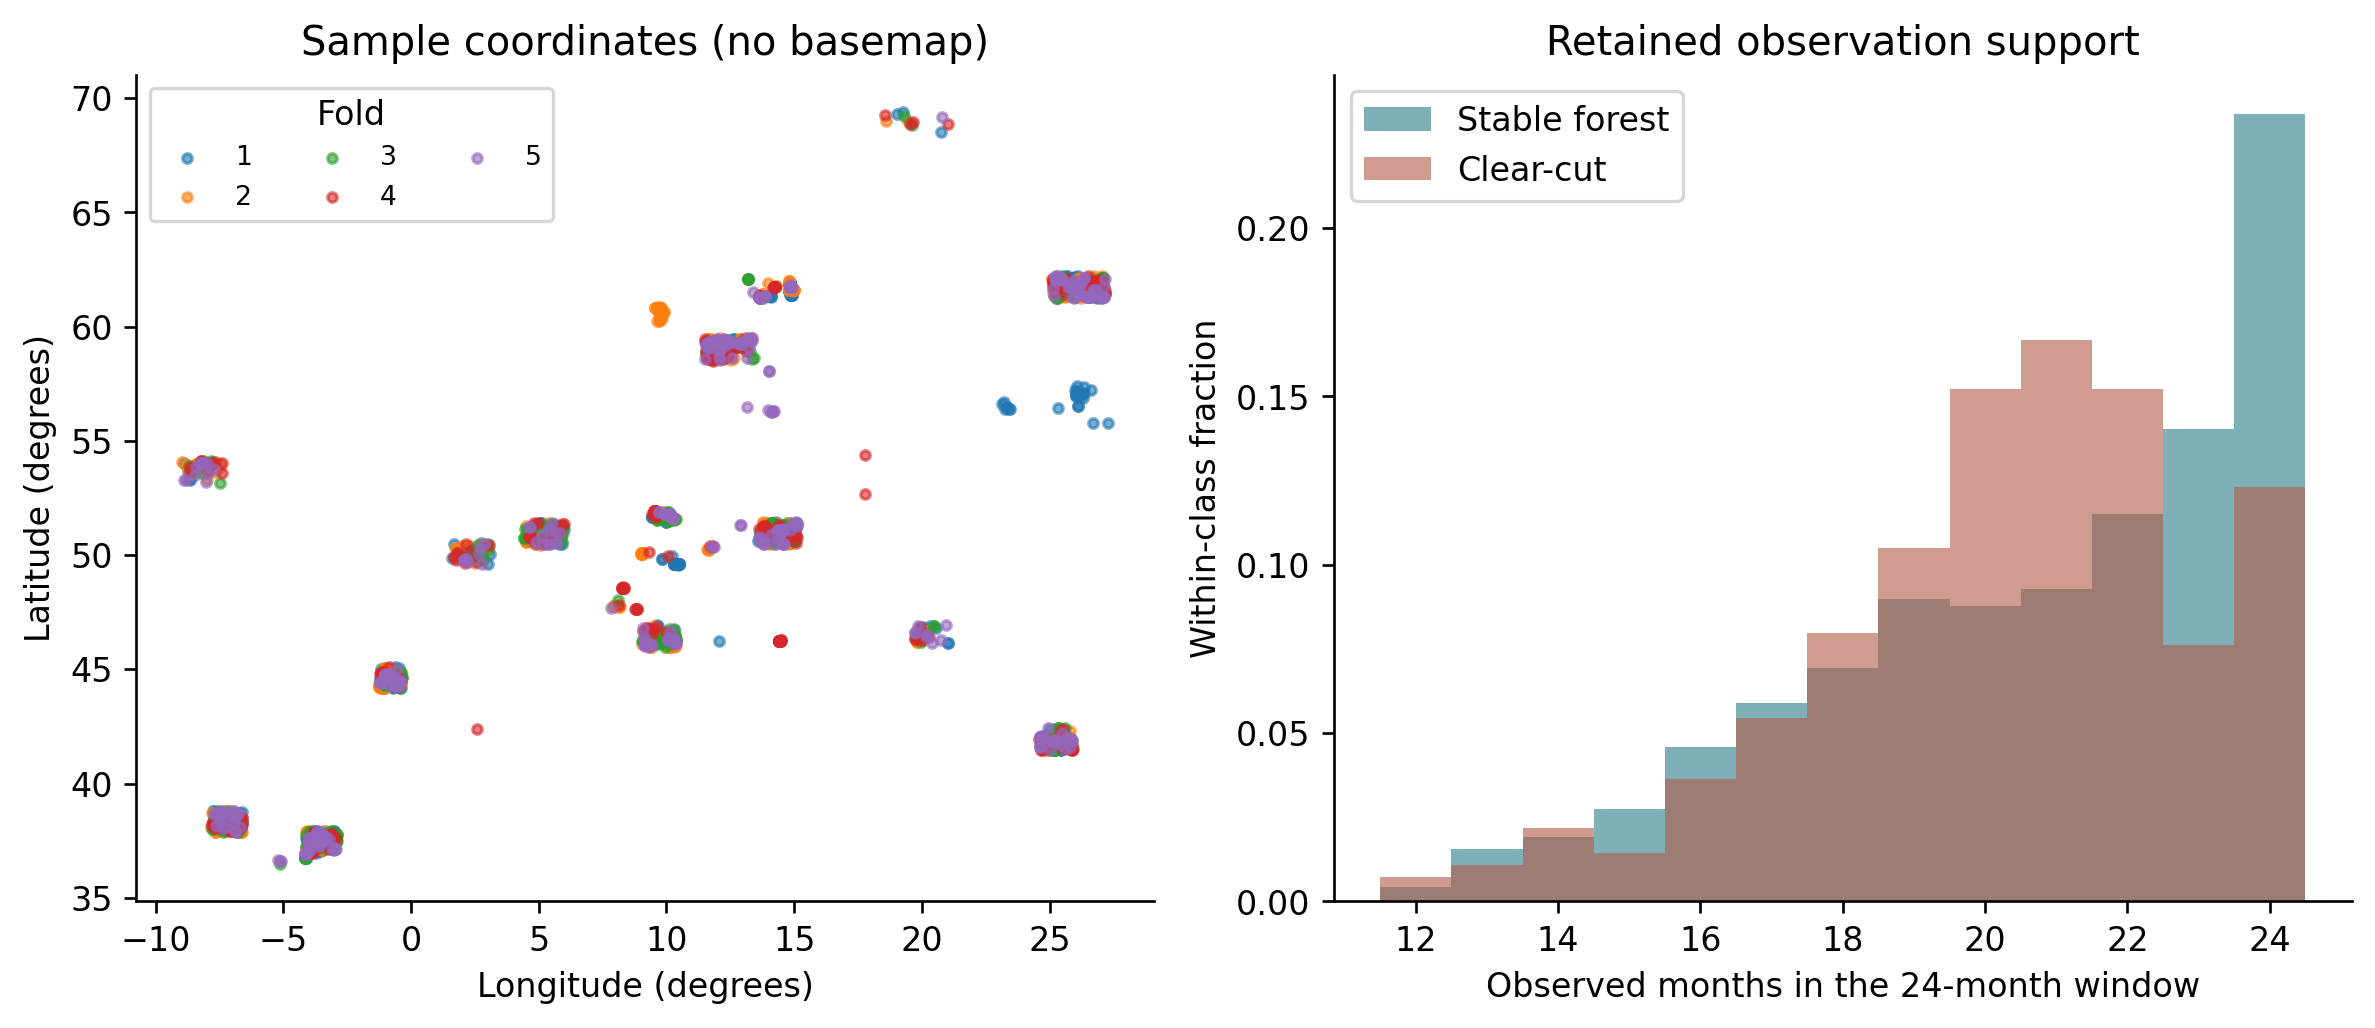
\includegraphics[width=\linewidth]{figures/03_data.png}
\caption{Locations and observed month support of the retained cohort. Colors identify the five fixed outer folds. Coordinates are plotted without a geographic basemap or area interpretation. Histograms are normalized separately within each class.}
\label{figure1}
\end{figure}

\begin{figure}[htbp]
\centering
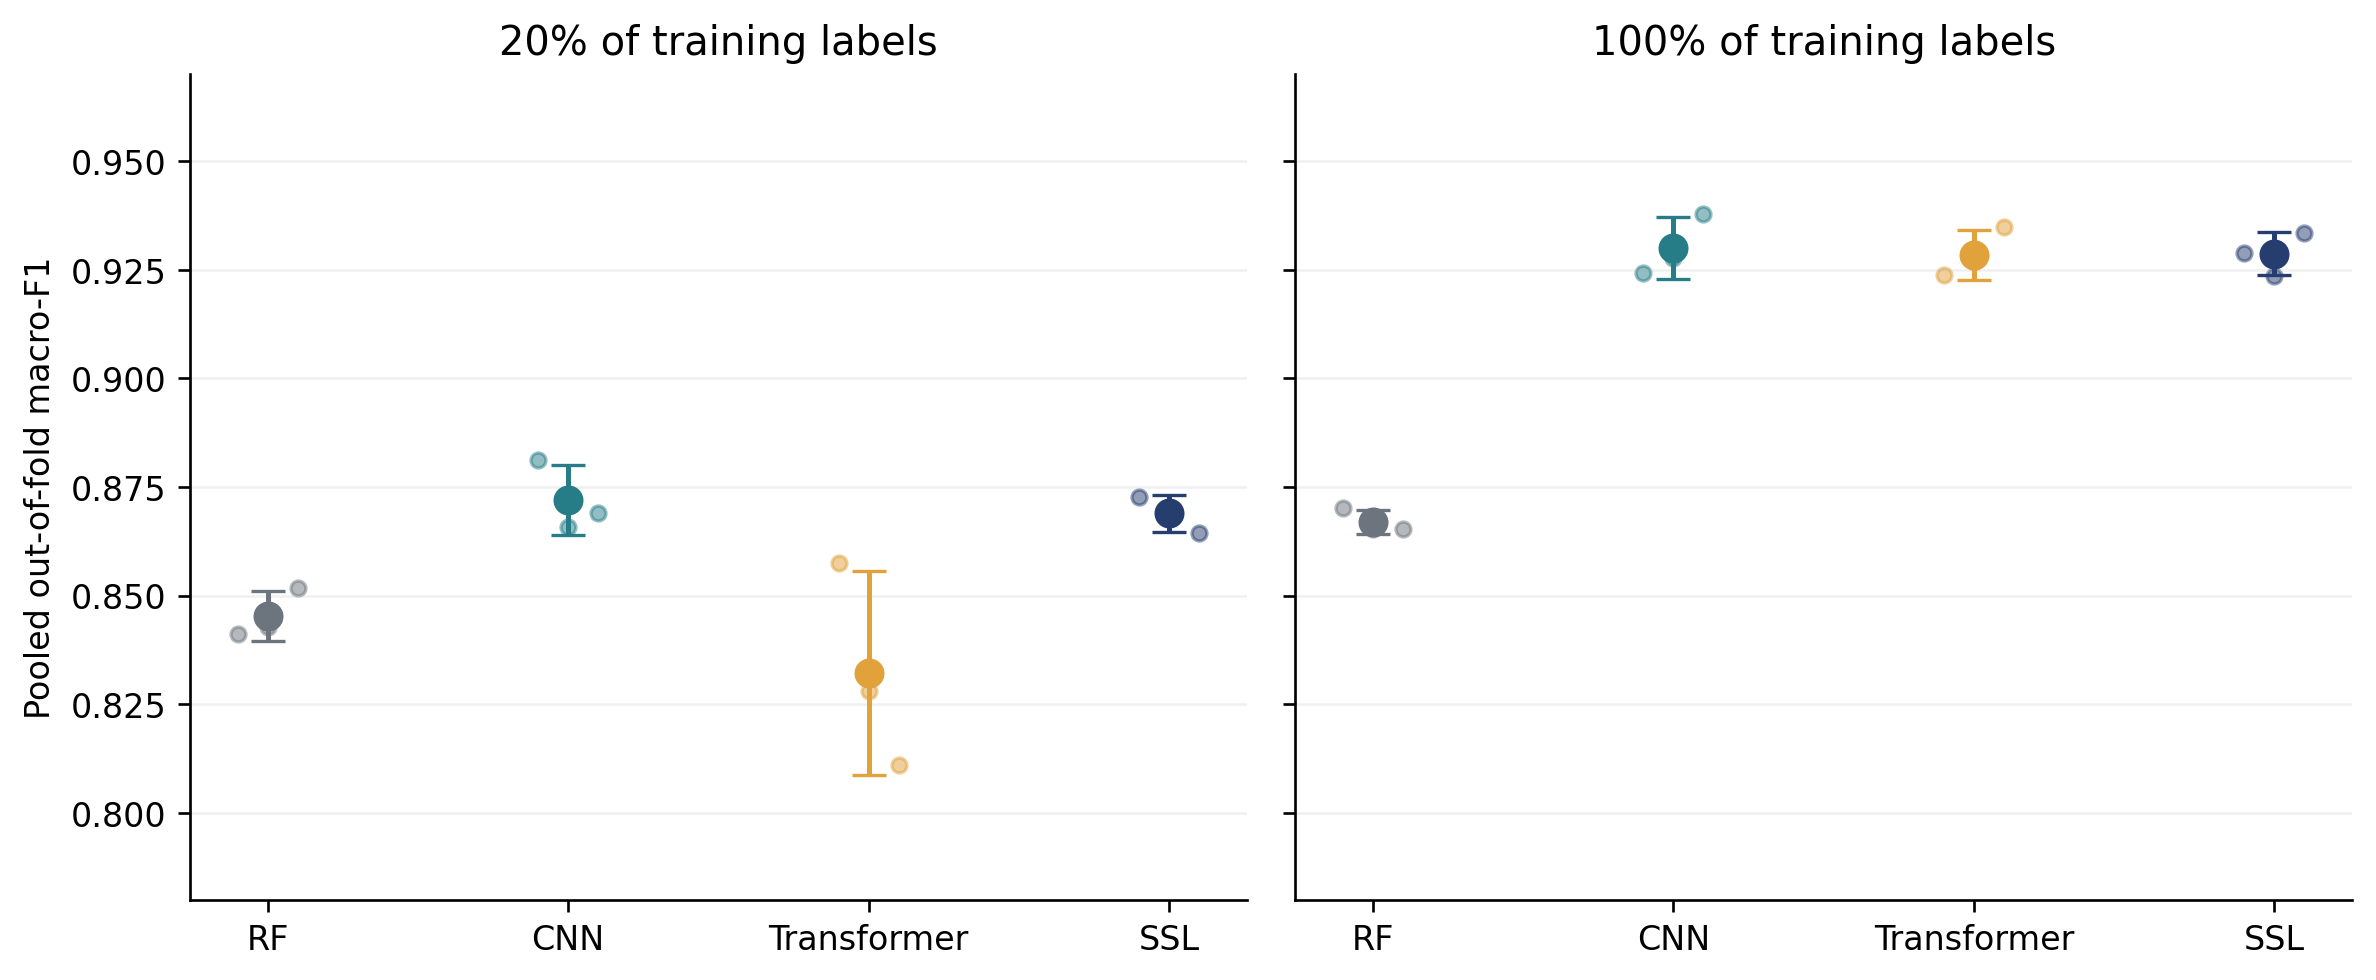
\includegraphics[width=\linewidth]{figures/01_primary.png}
\caption{Primary comparisons at 20\% and 100\% training labels. Large points are means of three pooled out of fold macro F1 values; error bars show their sample standard deviations. Smaller points are individual seeds. These bars are seed standard deviations rather than confidence intervals.}
\label{figure2}
\end{figure}

\begin{figure}[htbp]
\centering
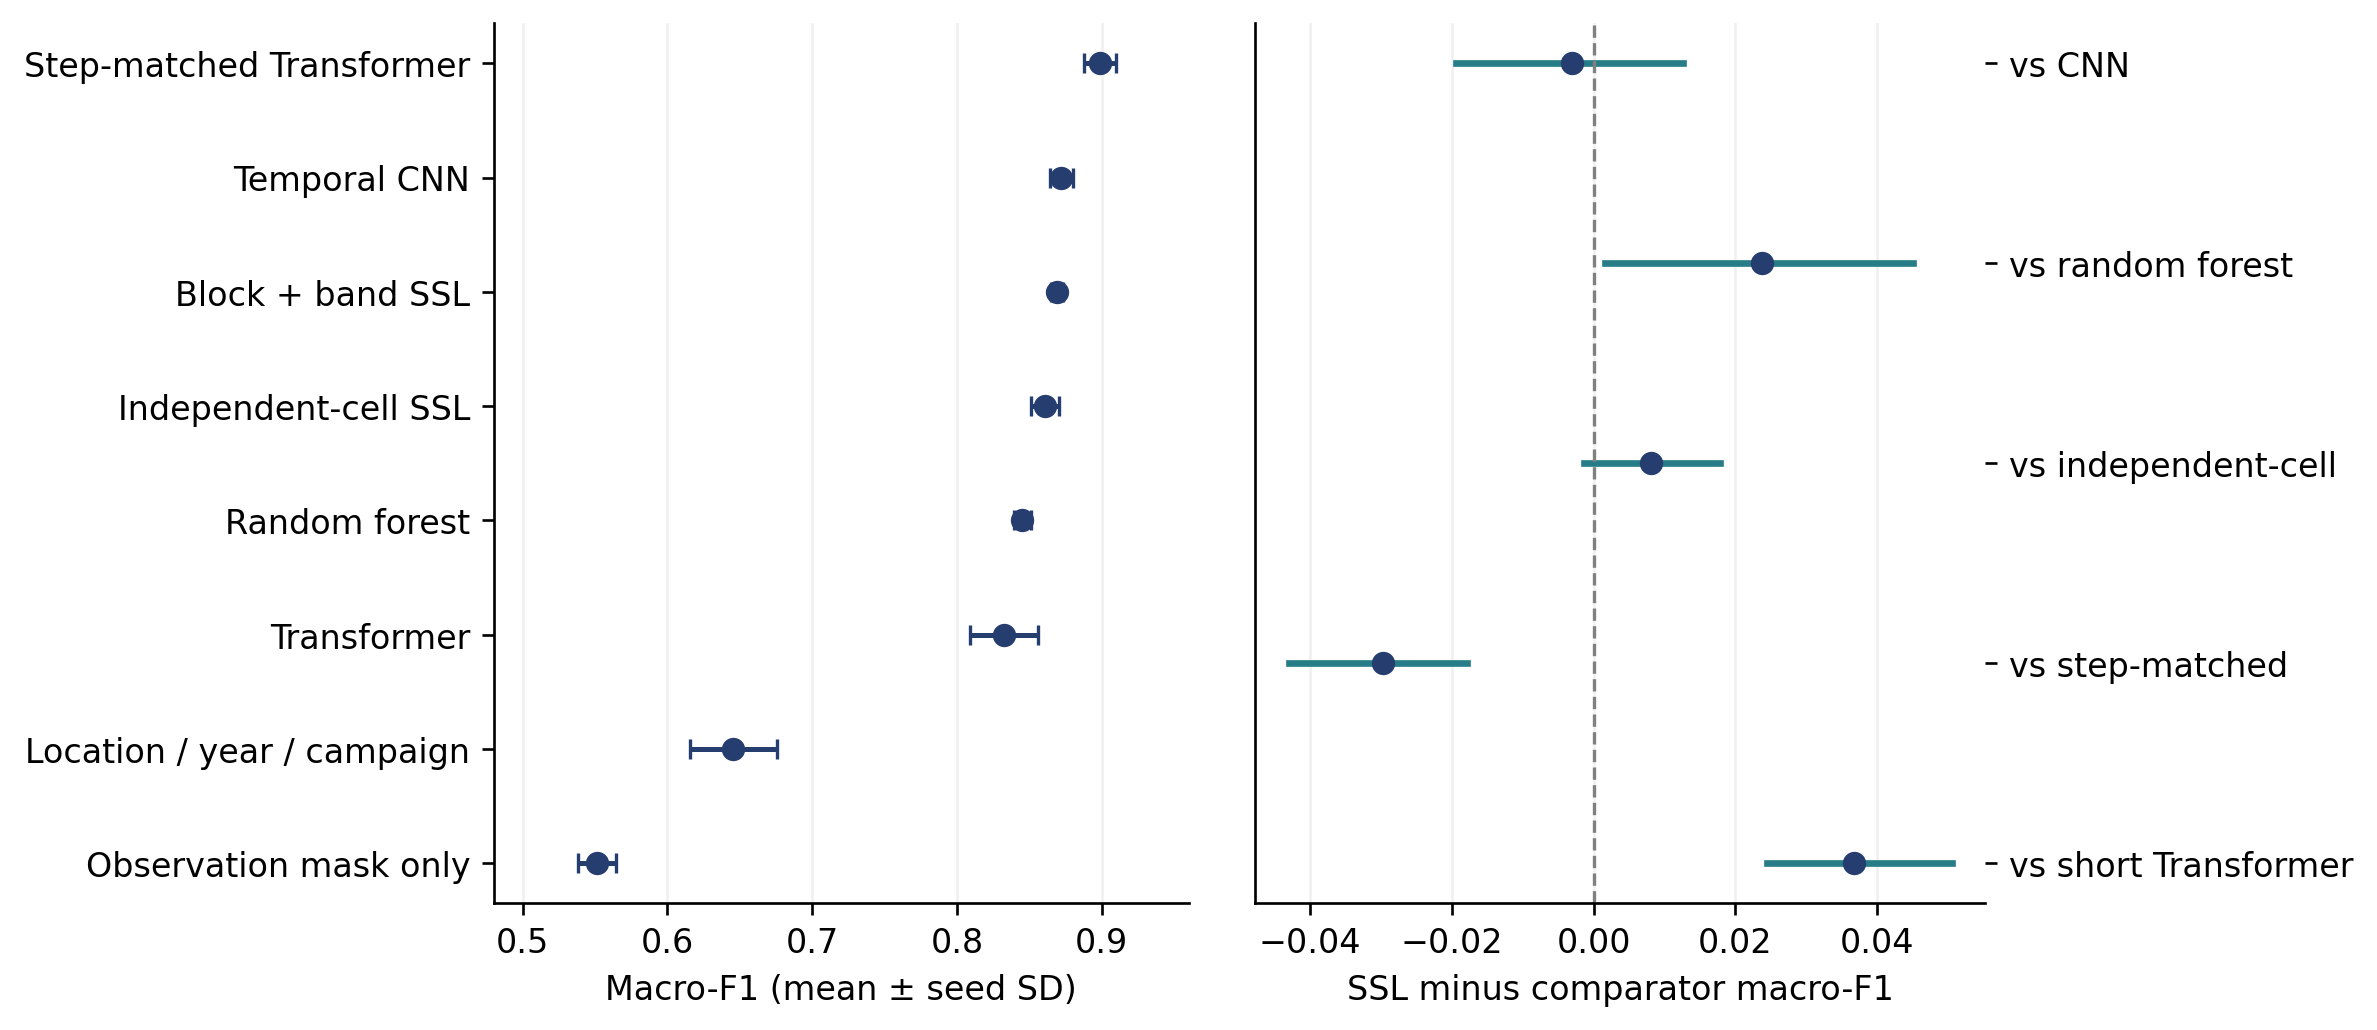
\includegraphics[width=\linewidth]{figures/02_controls.png}
\caption{Low label controls and paired comparisons. Left: macro F1 mean and seed standard deviation. Right: SSL minus comparator differences with 2,000 draw paired spatial component bootstrap percentile intervals. Only the short Transformer contrast is primary; other intervals are exploratory and conditional on the fixed fits.}
\label{figure3}
\end{figure}

\begin{figure}[htbp]
\centering
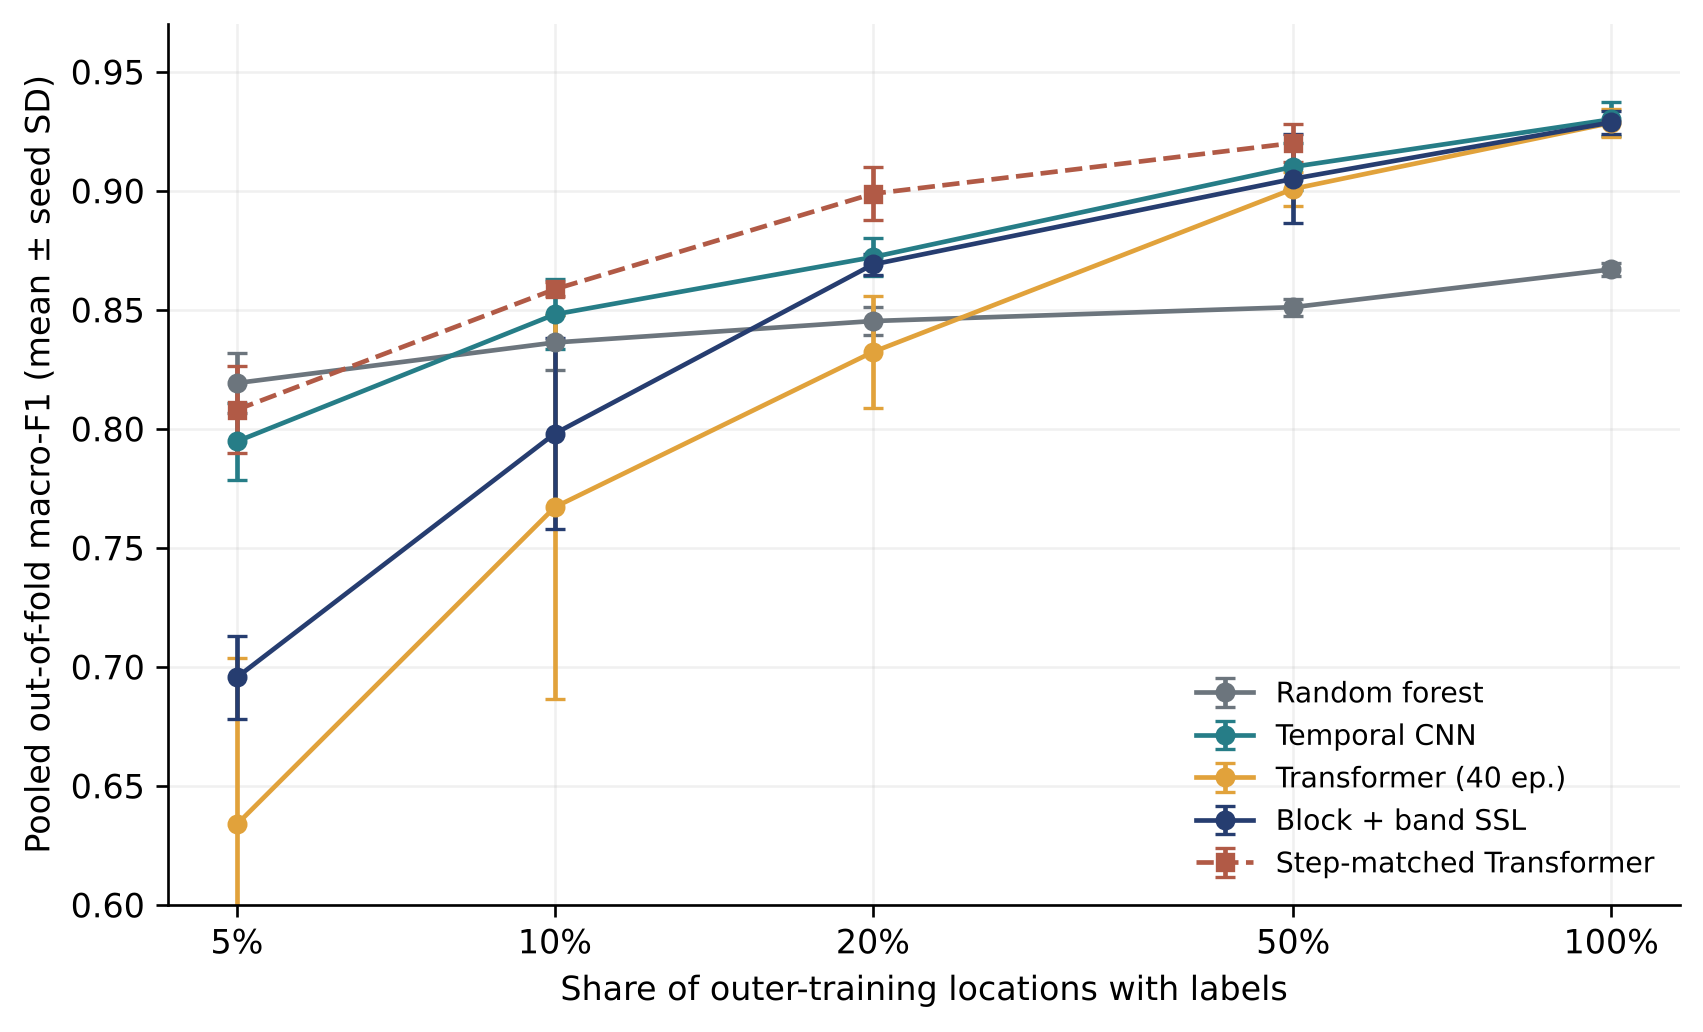
\includegraphics[width=\linewidth]{figures/04_label_curve.png}
\caption{Label budget curve on the frozen folds. Points are means of three pooled out of fold macro F1 values; bars are seed standard deviations and should not be read as confidence intervals. The 20\% and 100\% points are the paper\_v4 fits; 5\%, 10\% and 50\% are the declared paper\_v6 fits.}
\label{figure4}
\end{figure}

\begin{figure}[htbp]
\centering
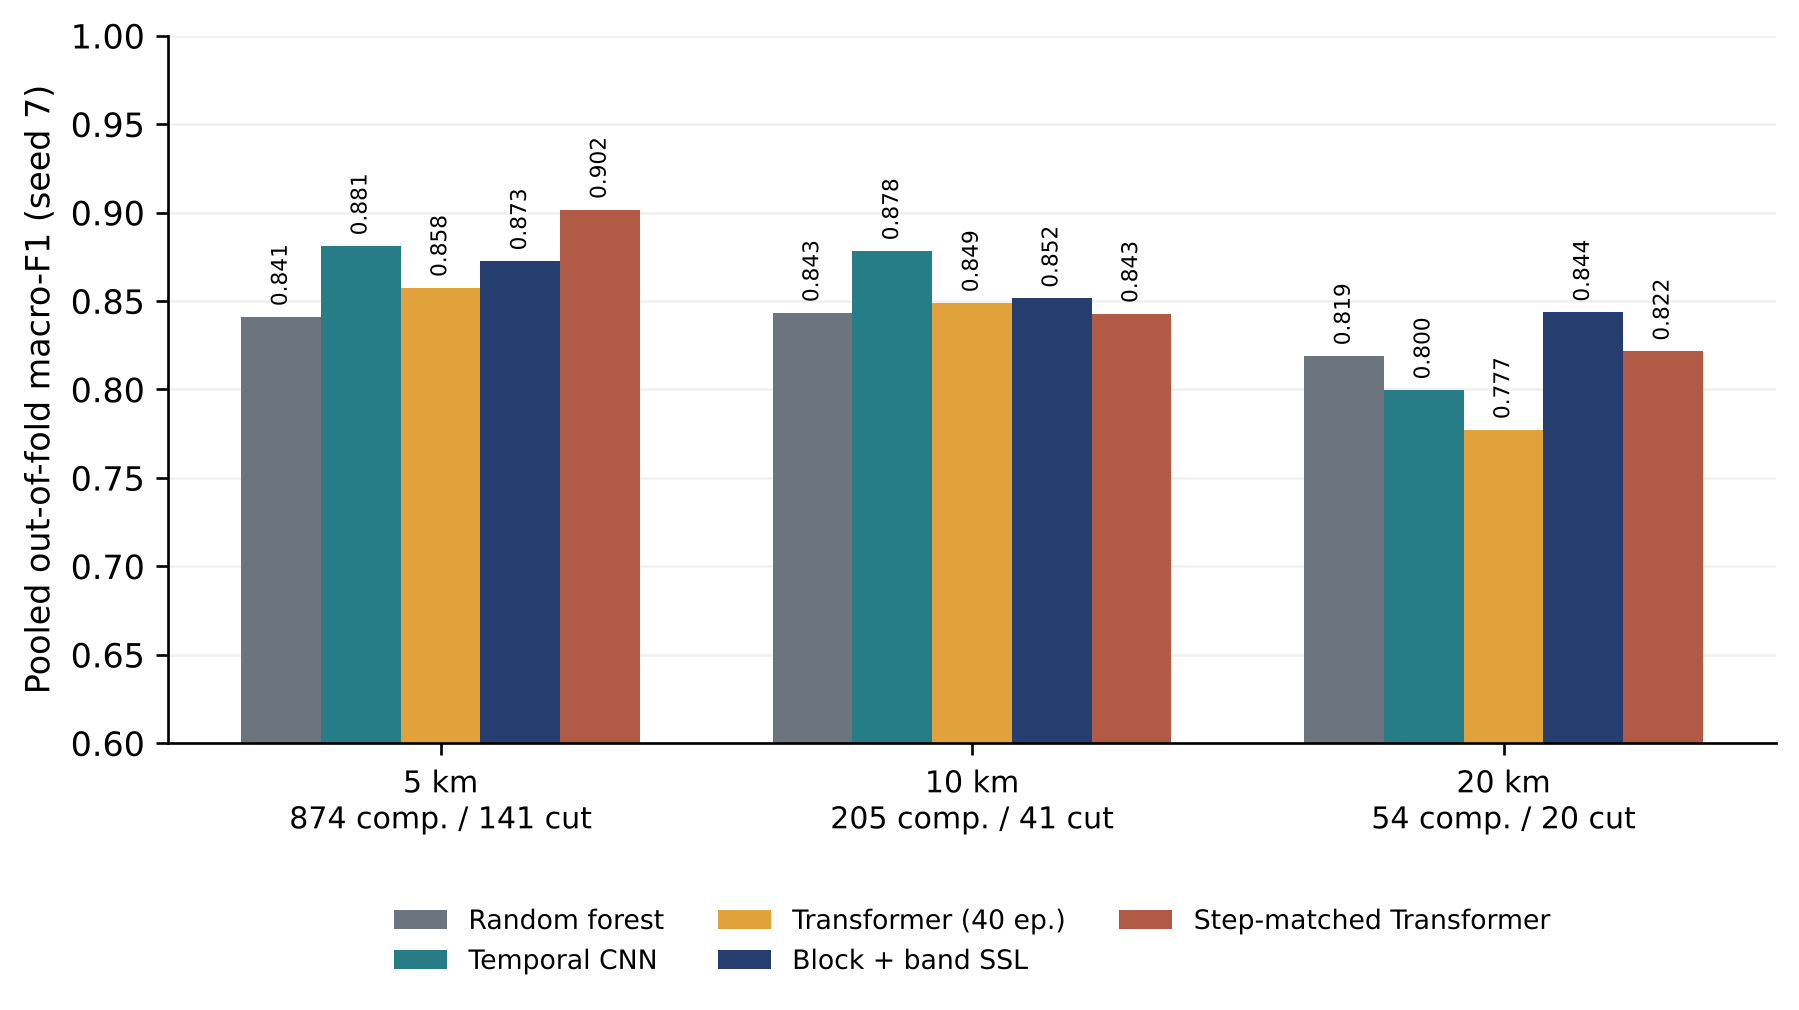
\includegraphics[width=\linewidth]{figures/05_radius.png}
\caption{Grouping radius sensitivity at 20\% labels, seed 7 only. Each bar is a single pooled out of fold macro F1; the number of spatial components and clear cut components per radius is given below the axis. Descriptive only.}
\label{figure5}
\end{figure}


\begin{thebibliography}{99}
\small
\bibitem{ref1} Viehweger, J.; Hirschmugl, M.; Puhm, M.; Burtscher, R.; Gallaun, H.; Deutscher, J. (2026). Dense labelled time series for mapping European forest disturbance agents. Earth System Science Data Discussions, preprint under review. \url{https://doi.org/10.5194/essd-2026-185}
\bibitem{ref2} Zhang, M.; Li, G.; Lu, D.; Xu, C.; Zhao, H.; Li, D. (2025). Self supervised deep learning for detection of forest disturbance types in a subtropical ecosystem using transformer and Sentinel 1 and Sentinel 2 time series data. International Journal of Digital Earth, 18, article 2537325. \url{https://doi.org/10.1080/17538947.2025.2537325}
\bibitem{ref3} Zerveas, G.; Jayaraman, S.; Patel, D.; Bhamidipaty, A.; Eickhoff, C. (2021). A Transformer based Framework for Multivariate Time Series Representation Learning. Proceedings of the 27th ACM SIGKDD Conference on Knowledge Discovery and Data Mining. \url{https://doi.org/10.1145/3447548.3467401}
\bibitem{ref4} Roberts, D. R.; Bahn, V.; Ciuti, S.; Boyce, M. S.; Elith, J.; Guillera Arroita, G.; Hauenstein, S.; Lahoz Monfort, J. J.; Schroder, B.; Thuiller, W.; Warton, D. I.; Wintle, B. A.; Hartig, F.; Dormann, C. F. (2017). Cross validation strategies for data with temporal, spatial, hierarchical, or phylogenetic structure. Ecography, 40, 913 to 929. \url{https://doi.org/10.1111/ecog.02881}
\bibitem{ref5} Breiman, L. (2001). Random Forests. Machine Learning, 45, 5 to 32. \url{https://doi.org/10.1023/A:1010933404324}
\bibitem{ref6} Guo, C.; Pleiss, G.; Sun, Y.; Weinberger, K. Q. (2017). On Calibration of Modern Neural Networks. Proceedings of Machine Learning Research, 70, 1321 to 1330. \url{https://proceedings.mlr.press/v70/guo17a.html}
\bibitem{ref7} Tseng, G.; Cartuyvels, R.; Zvonkov, I.; Purohit, M.; Rolnick, D.; Kerner, H. (2024). Lightweight, Pre trained Transformers for Remote Sensing Timeseries. arXiv:2304.14065, version 4. \url{https://doi.org/10.48550/arXiv.2304.14065}
\bibitem{ref8} Saget, A.; Lafabregue, B.; Cornuejols, A.; Gancarski, P. (2025). Resampling Augmentation for Time Series Contrastive Learning: Application to Remote Sensing. Proceedings of the TerraBytes ICML Workshop, PMLR 292, 32 to 45. \url{https://proceedings.mlr.press/v292/saget25a.html}
\bibitem{ref9} Yuan, Y.; Lin, L. (2021). Self Supervised Pretraining of Transformers for Satellite Image Time Series Classification. IEEE Journal of Selected Topics in Applied Earth Observations and Remote Sensing, 14, 474 to 487. \url{https://doi.org/10.1109/JSTARS.2020.3036602}
\bibitem{ref10} Yuan, Y.; Lin, L.; Liu, Q.; Hang, R.; Zhou, Z. G. (2022). SITS Former: A pre trained spatio spectral temporal representation model for Sentinel 2 time series classification. International Journal of Applied Earth Observation and Geoinformation, 106, article 102651. \url{https://doi.org/10.1016/j.jag.2021.102651}
\bibitem{ref11} Pelletier, C.; Webb, G. I.; Petitjean, F. (2019). Temporal Convolutional Neural Network for the Classification of Satellite Image Time Series. Remote Sensing, 11(5), article 523. \url{https://doi.org/10.3390/rs11050523}
\bibitem{ref12} Rußwurm, M.; Körner, M. (2020). Self attention for raw optical Satellite Time Series Classification. ISPRS Journal of Photogrammetry and Remote Sensing, 169, 421 to 435. \url{https://doi.org/10.1016/j.isprsjprs.2020.06.006}
\bibitem{ref13} Sainte Fare Garnot, V.; Landrieu, L.; Giordano, S.; Chehata, N. (2020). Satellite Image Time Series Classification With Pixel Set Encoders and Temporal Self Attention. Proceedings of the IEEE/CVF Conference on Computer Vision and Pattern Recognition (CVPR), 12322 to 12331. \url{https://doi.org/10.1109/CVPR42600.2020.01234}
\bibitem{ref14} He, K.; Chen, X.; Xie, S.; Li, Y.; Dollár, P.; Girshick, R. (2022). Masked Autoencoders Are Scalable Vision Learners. Proceedings of the IEEE/CVF Conference on Computer Vision and Pattern Recognition (CVPR), 15979 to 15988. \url{https://doi.org/10.1109/CVPR52688.2022.01553}
\bibitem{ref15} Cong, Y.; Khanna, S.; Meng, C.; Liu, P.; Rozi, E.; He, Y.; Burke, M.; Lobell, D. B.; Ermon, S. (2022). SatMAE: Pre training Transformers for Temporal and Multi Spectral Satellite Imagery. arXiv:2207.08051 (Advances in Neural Information Processing Systems 35). \url{https://doi.org/10.48550/arXiv.2207.08051}
\bibitem{ref16} Jakubik, J.; Roy, S.; Phillips, C. E.; et al. (2023). Foundation Models for Generalist Geospatial Artificial Intelligence. arXiv:2310.18660. \url{https://doi.org/10.48550/arXiv.2310.18660}
\bibitem{ref17} Hansen, M. C.; Potapov, P. V.; Moore, R.; Hancher, M.; Turubanova, S. A.; Tyukavina, A.; Thau, D.; Stehman, S. V.; Goetz, S. J.; Loveland, T. R.; Kommareddy, A.; Egorov, A.; Chini, L.; Justice, C. O.; Townshend, J. R. G. (2013). High Resolution Global Maps of 21st Century Forest Cover Change. Science, 342(6160), 850 to 853. \url{https://doi.org/10.1126/science.1244693}
\bibitem{ref18} Senf, C.; Seidl, R. (2021). Mapping the forest disturbance regimes of Europe. Nature Sustainability, 4, 63 to 70. \url{https://doi.org/10.1038/s41893-020-00609-y}
\bibitem{ref19} Hirschmugl, M.; Gallaun, H.; Dees, M.; Datta, P.; Deutscher, J.; Koutsias, N.; Schardt, M. (2017). Methods for Mapping Forest Disturbance and Degradation from Optical Earth Observation Data: a Review. Current Forestry Reports, 3, 32 to 45. \url{https://doi.org/10.1007/s40725-017-0047-2}
\bibitem{ref20} Zhu, Z.; Woodcock, C. E. (2014). Continuous change detection and classification of land cover using all available Landsat data. Remote Sensing of Environment, 144, 152 to 171. \url{https://doi.org/10.1016/j.rse.2014.01.011}
\bibitem{ref21} Ploton, P.; Mortier, F.; Réjou Méchain, M.; Barbier, N.; Picard, N.; Rossi, V.; Dormann, C.; Cornu, G.; Viennois, G.; Bayol, N.; Lyapustin, A.; Gourlet Fleury, S.; Pélissier, R. (2020). Spatial validation reveals poor predictive performance of large scale ecological mapping models. Nature Communications, 11, article 4540. \url{https://doi.org/10.1038/s41467-020-18321-y}
\bibitem{ref22} Meyer, H.; Pebesma, E. (2022). Machine learning based global maps of ecological variables and the challenge of assessing them. Nature Communications, 13, article 2208. \url{https://doi.org/10.1038/s41467-022-29838-9}
\bibitem{ref23} Wadoux, A. M. J. C.; Heuvelink, G. B. M.; de Bruin, S.; Brus, D. J. (2021). Spatial cross validation is not the right way to evaluate map accuracy. Ecological Modelling, 457, article 109692. \url{https://doi.org/10.1016/j.ecolmodel.2021.109692}
\bibitem{ref24} Wang, L.; Liu, S.; Song, W.; Ding, S.; Zhang, J. (2026). Global high resolution forest disturbance type dataset. Earth System Science Data, 18, 1601 to 1617. \url{https://doi.org/10.5194/essd-18-1601-2026}
\bibitem{ref25} Maze, M.; Attaher, S.; Taqi, M. O.; Elsawy, R.; Gad El Moula, M. M. H.; Hashem, F. A.; Moussa, A. S. (2025). Enhanced agricultural land use/land cover classification in the Nile Delta using Sentinel 1 and Sentinel 2 data and machine learning. ISPRS Journal of Photogrammetry and Remote Sensing, 229, 239 to 253. \url{https://doi.org/10.1016/j.isprsjprs.2025.08.019}
\bibitem{ref26} Vyas, N.; Singh, S.; Sethi, G. K. (2025). A novel image fusion based post classification framework for agricultural variations detection using Sentinel 1 and Sentinel 2 data. Earth Science Informatics, 18, article 40 (online 2024). \url{https://doi.org/10.1007/s12145-024-01506-0}
\end{thebibliography}
\end{document}
